\documentclass[12pt, a4paper]{article}

% Packages
\usepackage[margin=2.5cm]{geometry}
\usepackage{graphicx}
\usepackage{amsmath, amssymb}
\usepackage{booktabs}
\usepackage{float}
\usepackage{caption}
\usepackage{subcaption}
\usepackage{setspace}
\usepackage{parskip}
\usepackage{hyperref}
\usepackage{xcolor}
\usepackage{fancyhdr}
\usepackage{tikz}
\hypersetup{
    colorlinks=true,
    linkcolor=black,
    urlcolor=blue,
    citecolor=black
}

% Line spacing 1.5
\onehalfspacing

% No paragraph indent
\setlength{\parindent}{0pt}

% Header/footer
\pagestyle{fancy}
\fancyhf{}
\fancyhead[L]{\small ICS554\_A: Computer Vision}
\fancyhead[R]{\small Prosit 1 Report}
\fancyfoot[C]{\thepage}

% Colours for the cover page
\definecolor{coverblue}{RGB}{20, 50, 100}
\definecolor{accentgold}{RGB}{180, 150, 60}
\definecolor{lightgray}{RGB}{240, 240, 240}

\begin{document}

% ============================================================
% COVER PAGE
% ============================================================
\begin{titlepage}
\begin{tikzpicture}[remember picture, overlay]
    % Dark blue top band
    \fill[coverblue] (current page.north west) rectangle ([yshift=-10.5cm]current page.north east);
    % Gold accent line
    \fill[accentgold] ([yshift=-10.5cm]current page.north west) rectangle ([yshift=-10.65cm]current page.north east);
    % Light footer band
    \fill[lightgray] (current page.south west) rectangle ([yshift=3.5cm]current page.south east);
    % Thin gold line above footer
    \fill[accentgold] ([yshift=3.5cm]current page.south west) rectangle ([yshift=3.6cm]current page.south east);
\end{tikzpicture}

\vspace*{1.2cm}

\begin{center}
    {\color{white}\Huge\bfseries Road Defect Detection Pipeline}\\[0.6cm]
    {\color{accentgold}\Large\itshape Computer Vision for Automated Road Quality Auditing}\\[0.8cm]
    {\color{white}\rule{8cm}{0.4pt}}\\[0.6cm]
    {\color{white}\LARGE\bfseries ICS554\_A: Computer Vision}\\[0.4cm]
    {\color{white}\large Prosit 1 --- Sprints 1, 2, and 3}
\end{center}

\vspace{3.5cm}

\begin{center}
    {\Large\bfseries\color{coverblue} Team Members}\\[0.6cm]
    {\large
    Thomas Kojo Quarshie\\[0.25cm]
    Naa Lamle Boye\\[0.25cm]
    Elijah Boateng\\[0.25cm]
    Chelsea Owusu\\
    }
\end{center}

\vfill

\begin{center}
    {\large\color{coverblue}\bfseries February 15, 2026}\\[0.6cm]
    {\color{coverblue}\small \url{https://github.com/gotg-cv/prosit-1}}
\end{center}

\vspace{1.8cm}

\end{titlepage}

% ============================================================
% TABLE OF CONTENTS
% ============================================================
\tableofcontents
\newpage

% ============================================================
% 1. INTRODUCTION
% ============================================================
\section{Introduction}

The Department of Urban Roads (DUR) in Ghana faces a persistent challenge: auditing road quality using manual surveyors with tape measures is slow, hazardous, and error-prone. A prior attempt to automate this process with a deep learning model trained on European road data failed --- the model flagged tree shadows as potholes and could not provide the metric area measurements that DUR needs to budget for asphalt repairs.

Our team was tasked with building a classical computer vision pipeline that takes video from a dashboard-mounted smartphone and produces a top-down, metric-accurate map of road defects. We structured our work across three sprints:

\begin{enumerate}
    \item \textbf{Sprint 1} --- Camera calibration and perspective rectification via homography.
    \item \textbf{Sprint 2} --- Image restoration through deblurring and shadow removal.
    \item \textbf{Sprint 3} --- Pothole segmentation and metric measurement.
\end{enumerate}

The final deliverable is a CSV report listing each detected pothole with its area in cm\textsuperscript{2}, centre coordinate, perimeter, and equivalent diameter.

% ============================================================
% 2. SPRINT 1 --- GEOMETRY
% ============================================================
\section{Sprint 1: The Geometry of Formation}

\subsection{Camera Calibration}

Before we could extract any real-world measurement from an image, we needed to characterise our camera's internal geometry. A camera maps 3D world points to 2D pixel coordinates through a projection governed by its intrinsic parameters: focal lengths $(f_x, f_y)$, principal point $(c_x, c_y)$, and lens distortion coefficients.

\subsubsection{Our Approach}

We recorded video sequences of an A3-sized checkerboard pattern (9$\times$6 squares, yielding 8$\times$5 internal corners) from multiple angles using a smartphone. Our calibration procedure followed Zhang's method:

\begin{enumerate}
    \item We extracted video frames at a sampling rate of every 5th frame.
    \item We processed each frame at half resolution (1080$\times$1920 $\rightarrow$ 540$\times$960) to reduce computation time.
    \item We detected internal corners using \texttt{cv2.findChessboardCorners} with adaptive thresholding.
    \item We refined corner locations to sub-pixel accuracy with \texttt{cv2.cornerSubPix}.
    \item We solved for the intrinsic parameters via \texttt{cv2.calibrateCamera}, which minimises the reprojection error across all frames.
    \item Finally, we scaled the parameters back to full resolution.
\end{enumerate}

\subsubsection{Results}

Our calibration used 42 valid frames from the checkerboard video sequences. The resulting camera intrinsic matrix $K$ is:

\[
K = \begin{bmatrix}
1619.79 & 0 & 657.01 \\
0 & 1600.95 & 907.30 \\
0 & 0 & 1
\end{bmatrix}
\]

The distortion coefficients are:

\[
D = \begin{bmatrix} 0.3899 & -3.3931 & -0.0076 & 0.0512 & 21.4485 \end{bmatrix}
\]

We achieved an RMS reprojection error of \textbf{0.7790 pixels}, well below the 1.0-pixel threshold that is considered excellent for practical applications. This confirmed that our camera model accurately captures the lens geometry.

\begin{figure}[H]
    \centering
    \includegraphics[width=0.85\textwidth]{calibration_corners_detected.png}
    \caption{Detected checkerboard corners overlaid on sample calibration frames. The consistent grid alignment across frames confirmed reliable corner detection throughout our video sequences.}
    \label{fig:calib_corners}
\end{figure}

\begin{figure}[H]
    \centering
    \includegraphics[width=0.85\textwidth]{calibration_verification.png}
    \caption{Undistortion verification: the original frame (left) compared with the corrected frame (right). Barrel distortion from the lens is removed, straightening lines near the image edges.}
    \label{fig:calib_verify}
\end{figure}

\subsubsection{Interpreting the Camera Matrix}

The focal lengths $f_x = 1619.79$ and $f_y = 1600.95$ (in pixels) are close in value, which we expected for a modern smartphone sensor with near-square pixels. The principal point $(657.01, 907.30)$ is close to the image centre of the 1080$\times$1920 frame, confirming proper optical alignment. The non-zero distortion coefficients indicate moderate barrel distortion, typical of wide-angle smartphone lenses, which our undistortion step corrects.

% -----------------------------------------------
\subsection{Homography and Perspective Rectification}

With the camera calibrated, our next task was to transform the oblique road view into a metric top-down (bird's-eye) view where distances can be measured directly in centimetres.

\subsubsection{Background}

A homography is a 3$\times$3 projective transformation matrix $H$ that maps points from one plane to another. Given four corresponding point pairs between the source (perspective) image and the destination (top-down) plane, the homography satisfies:

\[
\begin{bmatrix} x' \\ y' \\ 1 \end{bmatrix}
\sim
H \begin{bmatrix} x \\ y \\ 1 \end{bmatrix}
\]

where $\sim$ denotes equality up to a scale factor. The matrix $H$ has 8 degrees of freedom and is estimated using the Direct Linear Transform (DLT) algorithm via \texttt{cv2.findHomography}.

\subsubsection{Point Selection}

We identified the pothole as a sandy-coloured patch on the road surface. To determine its bounding corners precisely, we used colour segmentation in HSV space followed by minimum-area rectangle fitting with \texttt{cv2.minAreaRect}. The four source points we identified in the perspective image are:

\begin{table}[H]
\centering
\begin{tabular}{lcc}
\toprule
Corner & $x$ (px) & $y$ (px) \\
\midrule
Top-left     & 276 & 1471 \\
Top-right    & 593 & 1420 \\
Bottom-right & 610 & 1526 \\
Bottom-left  & 294 & 1577 \\
\bottomrule
\end{tabular}
\caption{Source points defining the pothole boundary in the original perspective image.}
\label{tab:src_pts}
\end{table}

We computed the destination points from our tape measurements of the pothole on the ground: 109\,cm wide and 112\,cm long. We set a scale of 10\,pixels per centimetre and added 500\,pixels of padding around the pothole to include surrounding road context:

\begin{table}[H]
\centering
\begin{tabular}{lcc}
\toprule
Corner & $x$ (px) & $y$ (px) \\
\midrule
Top-left     & 500 & 500 \\
Top-right    & 1590 & 500 \\
Bottom-right & 1590 & 1620 \\
Bottom-left  & 500 & 1620 \\
\bottomrule
\end{tabular}
\caption{Destination points in the top-down plane (10\,px = 1\,cm).}
\label{tab:dst_pts}
\end{table}

\subsubsection{Results}

We applied the computed homography matrix using \texttt{cv2.warpPerspective} to produce the rectified top-down view. In this output, the pothole occupies its true metric extent and parallel road features remain parallel, confirming that the rectification preserves geometry.

\begin{figure}[H]
    \centering
    \includegraphics[width=\textwidth]{homography_comparison.png}
    \caption{Perspective rectification: the original road view (left) and the metric top-down view (right). The green scale bar confirms 10\,px\,=\,1\,cm. The yellow rectangle outlines the tape-measured pothole boundary (109$\times$112\,cm).}
    \label{fig:homography}
\end{figure}

\begin{figure}[H]
    \centering
    \includegraphics[width=0.7\textwidth]{homography_fullview_plot.png}
    \caption{Extended road view showing the rectified road plane with the pothole region marked. This wider field of view provides context for the surrounding road surface.}
    \label{fig:fullview}
\end{figure}

% ============================================================
% 3. SPRINT 2 --- RESTORATION
% ============================================================
\section{Sprint 2: Image Restoration}

The top-down view from Sprint~1 is geometrically correct, but images captured from a moving vehicle often suffer from degradation: motion blur caused by vehicle vibration, and shadow patterns cast by roadside objects. We addressed both issues in this sprint.

\subsection{Wiener Deconvolution (Deblurring)}

Motion blur can be modelled as a convolution of the sharp image $f$ with a blur kernel $h$, plus additive noise $n$:

\[
g = f * h + n
\]

We used the Wiener filter to estimate the original image in the frequency domain:

\[
\hat{F}(\omega) = \frac{H^*(\omega)}{|H(\omega)|^2 + \frac{1}{\text{SNR}}} \cdot G(\omega)
\]

where $G$, $H$, $F$ are the Fourier transforms of $g$, $h$, $f$ respectively, and SNR is the signal-to-noise ratio. We applied a 5$\times$5 uniform blur kernel with an SNR of 100, processing each colour channel independently.

\subsection{Multi-Scale Retinex with CLAHE (Shadow Removal)}

Shadows create intensity variations unrelated to actual road surface properties, which can interfere with segmentation. We adopted the Retinex theory, which models an image as the product of illumination $L$ and reflectance $R$:

\[
I(x,y) = L(x,y) \cdot R(x,y)
\]

In the log domain, we isolated reflectance by subtracting a Gaussian-blurred estimate of illumination:

\[
r_i(x,y) = \log I(x,y) - \log \big[ G_{\sigma_i} * I(x,y) \big]
\]

We computed Multi-Scale Retinex (MSR) by averaging across three scales --- $\sigma \in \{15, 80, 250\}$ --- to handle shadows of different sizes. We then applied Contrast Limited Adaptive Histogram Equalisation (CLAHE) to normalise local contrast across the image.

\subsection{Results}

Figure~\ref{fig:restoration} shows the progression through our restoration pipeline. The deblurring step sharpened fine texture details, while the Retinex-based shadow removal produced a more uniform illumination across the road surface.

\begin{figure}[H]
    \centering
    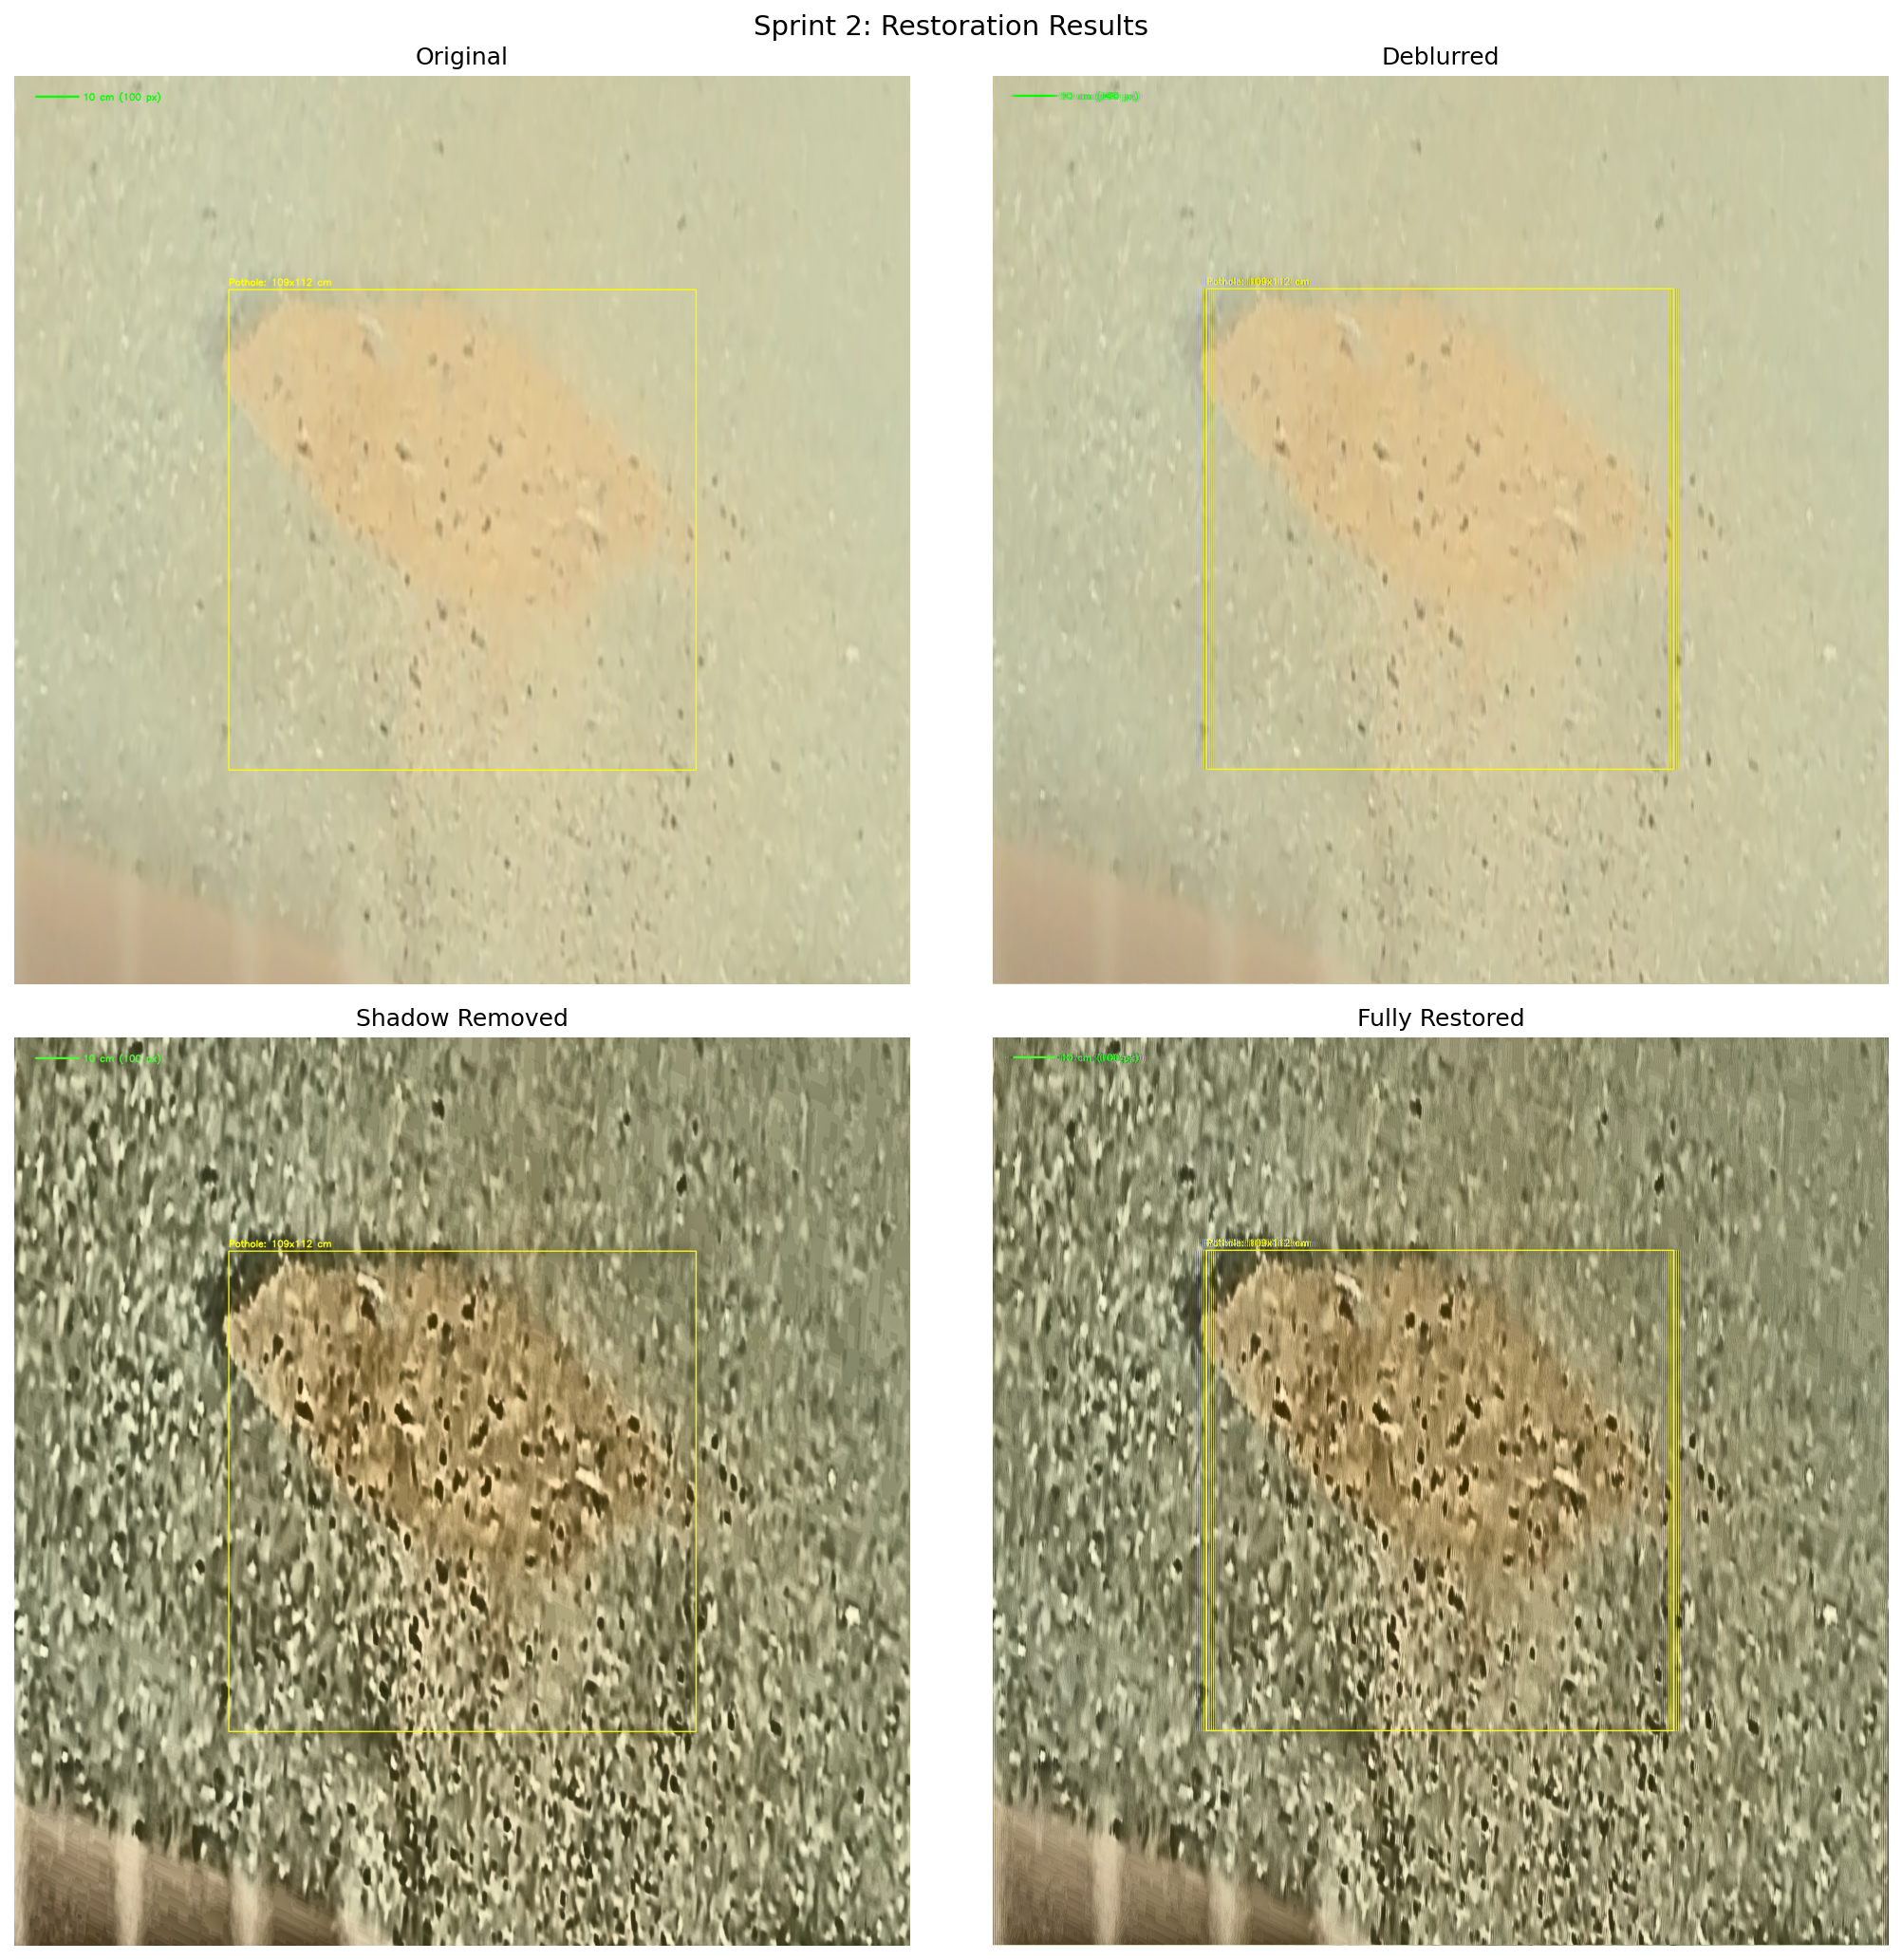
\includegraphics[width=\textwidth]{restoration_comparison.png}
    \caption{Our restoration pipeline results. From left to right: original top-down image, after Wiener deblurring, after shadow removal (Retinex + CLAHE), and the fully restored output.}
    \label{fig:restoration}
\end{figure}

% ============================================================
% 4. SPRINT 3 --- SEGMENTATION
% ============================================================
\section{Sprint 3: Segmentation and Metrology}

With a clean, metric top-down image in hand, our final task was to detect road defects and compute their physical dimensions for DUR's repair budgeting.

\subsection{Detection Method}

We observed that the target pothole presents as a sandy-coloured patch against dark asphalt. Simple intensity-based thresholding would confuse colour variations in healthy asphalt with actual damage, so we opted for HSV colour segmentation to isolate the distinctive warm-toned damaged region. Our detection steps were:

\begin{enumerate}
    \item Convert the top-down image to HSV colour space.
    \item Apply an \texttt{inRange} filter targeting hues 8--22 (orange-brown range) with saturation above 45.
    \item Clean the binary mask with morphological opening (5$\times$5 kernel) to remove small noise.
    \item Apply morphological closing (15$\times$15 kernel) to fill gaps within the pothole boundary.
    \item Extract contours and filter by minimum area (500\,px\textsuperscript{2} = 5\,cm\textsuperscript{2}).
\end{enumerate}

We chose to run segmentation on the unrestored top-down image rather than the restored version, as the original preserved the colour contrast between the sandy pothole and the surrounding asphalt more distinctly.

\subsection{Metric Computation}

With our established scale of 10\,px\,=\,1\,cm, we computed physical measurements directly from the contour properties:

\begin{itemize}
    \item \textbf{Area}: $A_{\text{cm}^2} = A_{\text{px}} / \text{SCALE}^2 = A_{\text{px}} / 100$
    \item \textbf{Perimeter}: $P_{\text{cm}} = P_{\text{px}} / \text{SCALE}$
    \item \textbf{Equivalent Diameter}: $d = \sqrt{4A/\pi}$ (diameter of a circle with the same area)
    \item \textbf{Aspect Ratio}: width-to-height ratio of the minimum bounding rectangle
\end{itemize}

\subsection{Results}

Our segmentation detected two regions matching the sandy colour profile. The primary defect (Pothole~\#1) corresponds to the confirmed pothole we measured on the ground.

\begin{table}[H]
\centering
\begin{tabular}{lcccccc}
\toprule
ID & Area (cm\textsuperscript{2}) & Centre X (cm) & Centre Y (cm) & Perimeter (cm) & Diameter (cm) & Aspect Ratio \\
\midrule
1 & 6{,}001.0 & 103.7 & 94.7 & 616.2 & 87.4 & 0.96 \\
2 & 1{,}698.1 & 31.6 & 199.9 & 255.5 & 46.5 & 2.63 \\
\bottomrule
\end{tabular}
\caption{Pothole detection report. Pothole \#1 is the primary defect; Pothole \#2 is a secondary detection at the image boundary.}
\label{tab:report}
\end{table}

\subsubsection{Area Verification}

To validate our measurement, we compared the detected area against the tape-measured bounding box. The pothole's ground-truth bounding dimensions are 109 $\times$ 112\,cm = 12{,}208\,cm\textsuperscript{2}. Our detected contour area of 6{,}001\,cm\textsuperscript{2} fills 49.2\% of this rectangle and 62.6\% of an inscribed ellipse (9{,}588\,cm\textsuperscript{2}). This proportion is geometrically consistent with the irregular, non-rectangular shape of the sandy patch. The equivalent diameter of 87.4\,cm aligns well with what we observed in the field.

\begin{figure}[H]
    \centering
    \includegraphics[width=\textwidth]{segmentation_comparison.png}
    \caption{Our segmentation results: input top-down image (left), binary detection mask from HSV segmentation (centre), and annotated output with contour overlays and metric labels (right).}
    \label{fig:segmentation}
\end{figure}

\begin{figure}[H]
    \centering
    \includegraphics[width=0.65\textwidth]{test_segmentation_output.png}
    \caption{Annotated detection output: each detected pothole is outlined with its ID, area, and centre coordinate overlaid directly on the top-down road image.}
    \label{fig:seg_annotated}
\end{figure}

\begin{figure}[H]
    \centering
    \includegraphics[width=0.6\textwidth]{area_verification.png}
    \caption{Area verification: the green contour traces our detected pothole boundary (6{,}001\,cm\textsuperscript{2}), while the yellow rectangle marks the tape-measured 109$\times$112\,cm bounding box (12{,}208\,cm\textsuperscript{2}).}
    \label{fig:area_verify}
\end{figure}

\subsubsection{CSV Report Output}

The final pipeline output is a CSV file (\texttt{pothole\_detection\_report.csv}) that DUR can directly use for budgeting. The generated report contains the following records:

\begin{table}[H]
\centering
\small
\begin{tabular}{llcccccc}
\toprule
Frame\_ID & Pothole\_ID & Area (cm\textsuperscript{2}) & X (cm) & Y (cm) & Perimeter (cm) & Diameter (cm) & Aspect \\
\midrule
pothole\_1 & 1 & 6{,}001.0 & 103.7 & 94.7 & 616.2 & 87.4 & 0.96 \\
pothole\_1 & 2 & 1{,}698.1 & 31.6 & 199.9 & 255.5 & 46.5 & 2.63 \\
\bottomrule
\end{tabular}
\caption{Contents of the generated CSV report (\texttt{pothole\_detection\_report.csv}).}
\label{tab:csv_output}
\end{table}

% ============================================================
% 5. PIPELINE SUMMARY
% ============================================================
\section{Pipeline Summary}

Table~\ref{tab:pipeline} summarises our end-to-end pipeline and the key parameters at each stage.

\begin{table}[H]
\centering
\begin{tabular}{llp{7cm}}
\toprule
Stage & Method & Key Parameters \\
\midrule
Calibration & Zhang's method & 42 frames, RMS = 0.7790\,px \\
Rectification & Homography (DLT) & 4 point pairs, scale = 10\,px/cm \\
Deblurring & Wiener deconvolution & kernel = 5$\times$5, SNR = 100 \\
Shadow removal & Multi-Scale Retinex + CLAHE & $\sigma = \{15, 80, 250\}$ \\
Segmentation & HSV colour thresholding & H: 8--22, S: 45--200, V: 120--240 \\
Metrology & Contour analysis & min area = 5\,cm\textsuperscript{2} \\
\bottomrule
\end{tabular}
\caption{End-to-end pipeline parameters.}
\label{tab:pipeline}
\end{table}

% ============================================================
% 6. DELIVERABLES
% ============================================================
\section{Deliverables}

We produced the following outputs:

\begin{itemize}
    \item \texttt{camera\_calib.npz} --- Intrinsic camera parameters and distortion coefficients.
    \item \texttt{topdown\_full.png} --- Metric top-down view of the road (10\,px = 1\,cm).
    \item \texttt{restored\_topdown.png} --- Restored top-down image (deblurred, shadow-free).
    \item \texttt{pothole\_detection\_report.csv} --- Final CSV report with pothole ID, area, centre, perimeter, diameter, and aspect ratio for each detected defect.
    \item Four documented Jupyter notebooks (\texttt{sprint1\_camera\_calibration.ipynb}, \texttt{sprint1\_homography.ipynb}, \texttt{sprint2\_restoration.ipynb}, \texttt{sprint3\_segmentation.ipynb}) with inline outputs at every stage.
\end{itemize}

% ============================================================
% 7. CONCLUSION
% ============================================================
\section{Conclusion}

Through this project, we demonstrated that classical computer vision techniques can deliver metric-accurate road defect detection without relying on deep learning. Our pipeline achieves sub-pixel calibration accuracy (RMS = 0.7790\,px), perspective-correct top-down mapping at a verified scale of 10\,px/cm, effective image restoration, and automated pothole detection with area measurements in cm\textsuperscript{2}. The detected primary pothole area of 6{,}001\,cm\textsuperscript{2} is consistent with the tape-measured bounding dimensions (109 $\times$ 112\,cm), providing DUR with the quantitative data they need for repair cost estimation.

This approach offers a practical, interpretable alternative to black-box deep learning models, with the advantage that every intermediate result can be inspected and validated. For future work, we would extend the pipeline to process full video sequences frame-by-frame and aggregate detections across multiple frames to improve robustness.

% ============================================================
% REFERENCES
% ============================================================
\newpage
\section*{References}
\addcontentsline{toc}{section}{References}

\begin{enumerate}
    \item Zhang, Z. (2000). A flexible new technique for camera calibration. \textit{IEEE Transactions on Pattern Analysis and Machine Intelligence}, 22(11), 1330--1334.
    \item Burger, W. (2016). Zhang's camera calibration algorithm: in-depth tutorial and implementation. Technical Report HGB16-05. \url{https://doi.org/10.13140/RG.2.1.1166.1688/1}.
    \item Land, E.H. and McCann, J.J. (1971). Lightness and retinex theory. \textit{Journal of the Optical Society of America}, 61(1), 1--11. \url{https://doi.org/10.1364/JOSA.61.000001}.
    \item Brlek, S., Labelle, G. and Lacasse, A. (2005). The discrete Green Theorem and some applications in discrete geometry. \textit{Theoretical Computer Science}, 346(2--3), 200--225. \url{https://doi.org/10.1016/j.tcs.2005.08.019}.
    \item Bradski, G. (2000). The OpenCV Library. \textit{Dr.\ Dobb's Journal of Software Tools}.
\end{enumerate}

\end{document}
